\section{Arduino kode}
Den indledende løsning blev først implementeret på en arduino uno hvor konceptet blev testet og verificeret.

\begin{figure}[h!]
  \centering
  \includegraphics[width=0.6\textwidth]{figures/followLine2.png}
  \caption{FollowLine() funtion.}
  \label{follow_line_kode}
\end{figure}

Koden fungerer sålades at  når sensoren registrere den hvide linje drejes der til højre og når den sorte linje registreres drejes der til venstre. Robotten kører derved kun på kanten af linjen.

\subsection{Test med én sensor}
Ud fra det introducerde linetrack system blev konceptet testet ved brug af én sensor på den opstillede bane. 

\begin{figure}[h!]
  \centering
  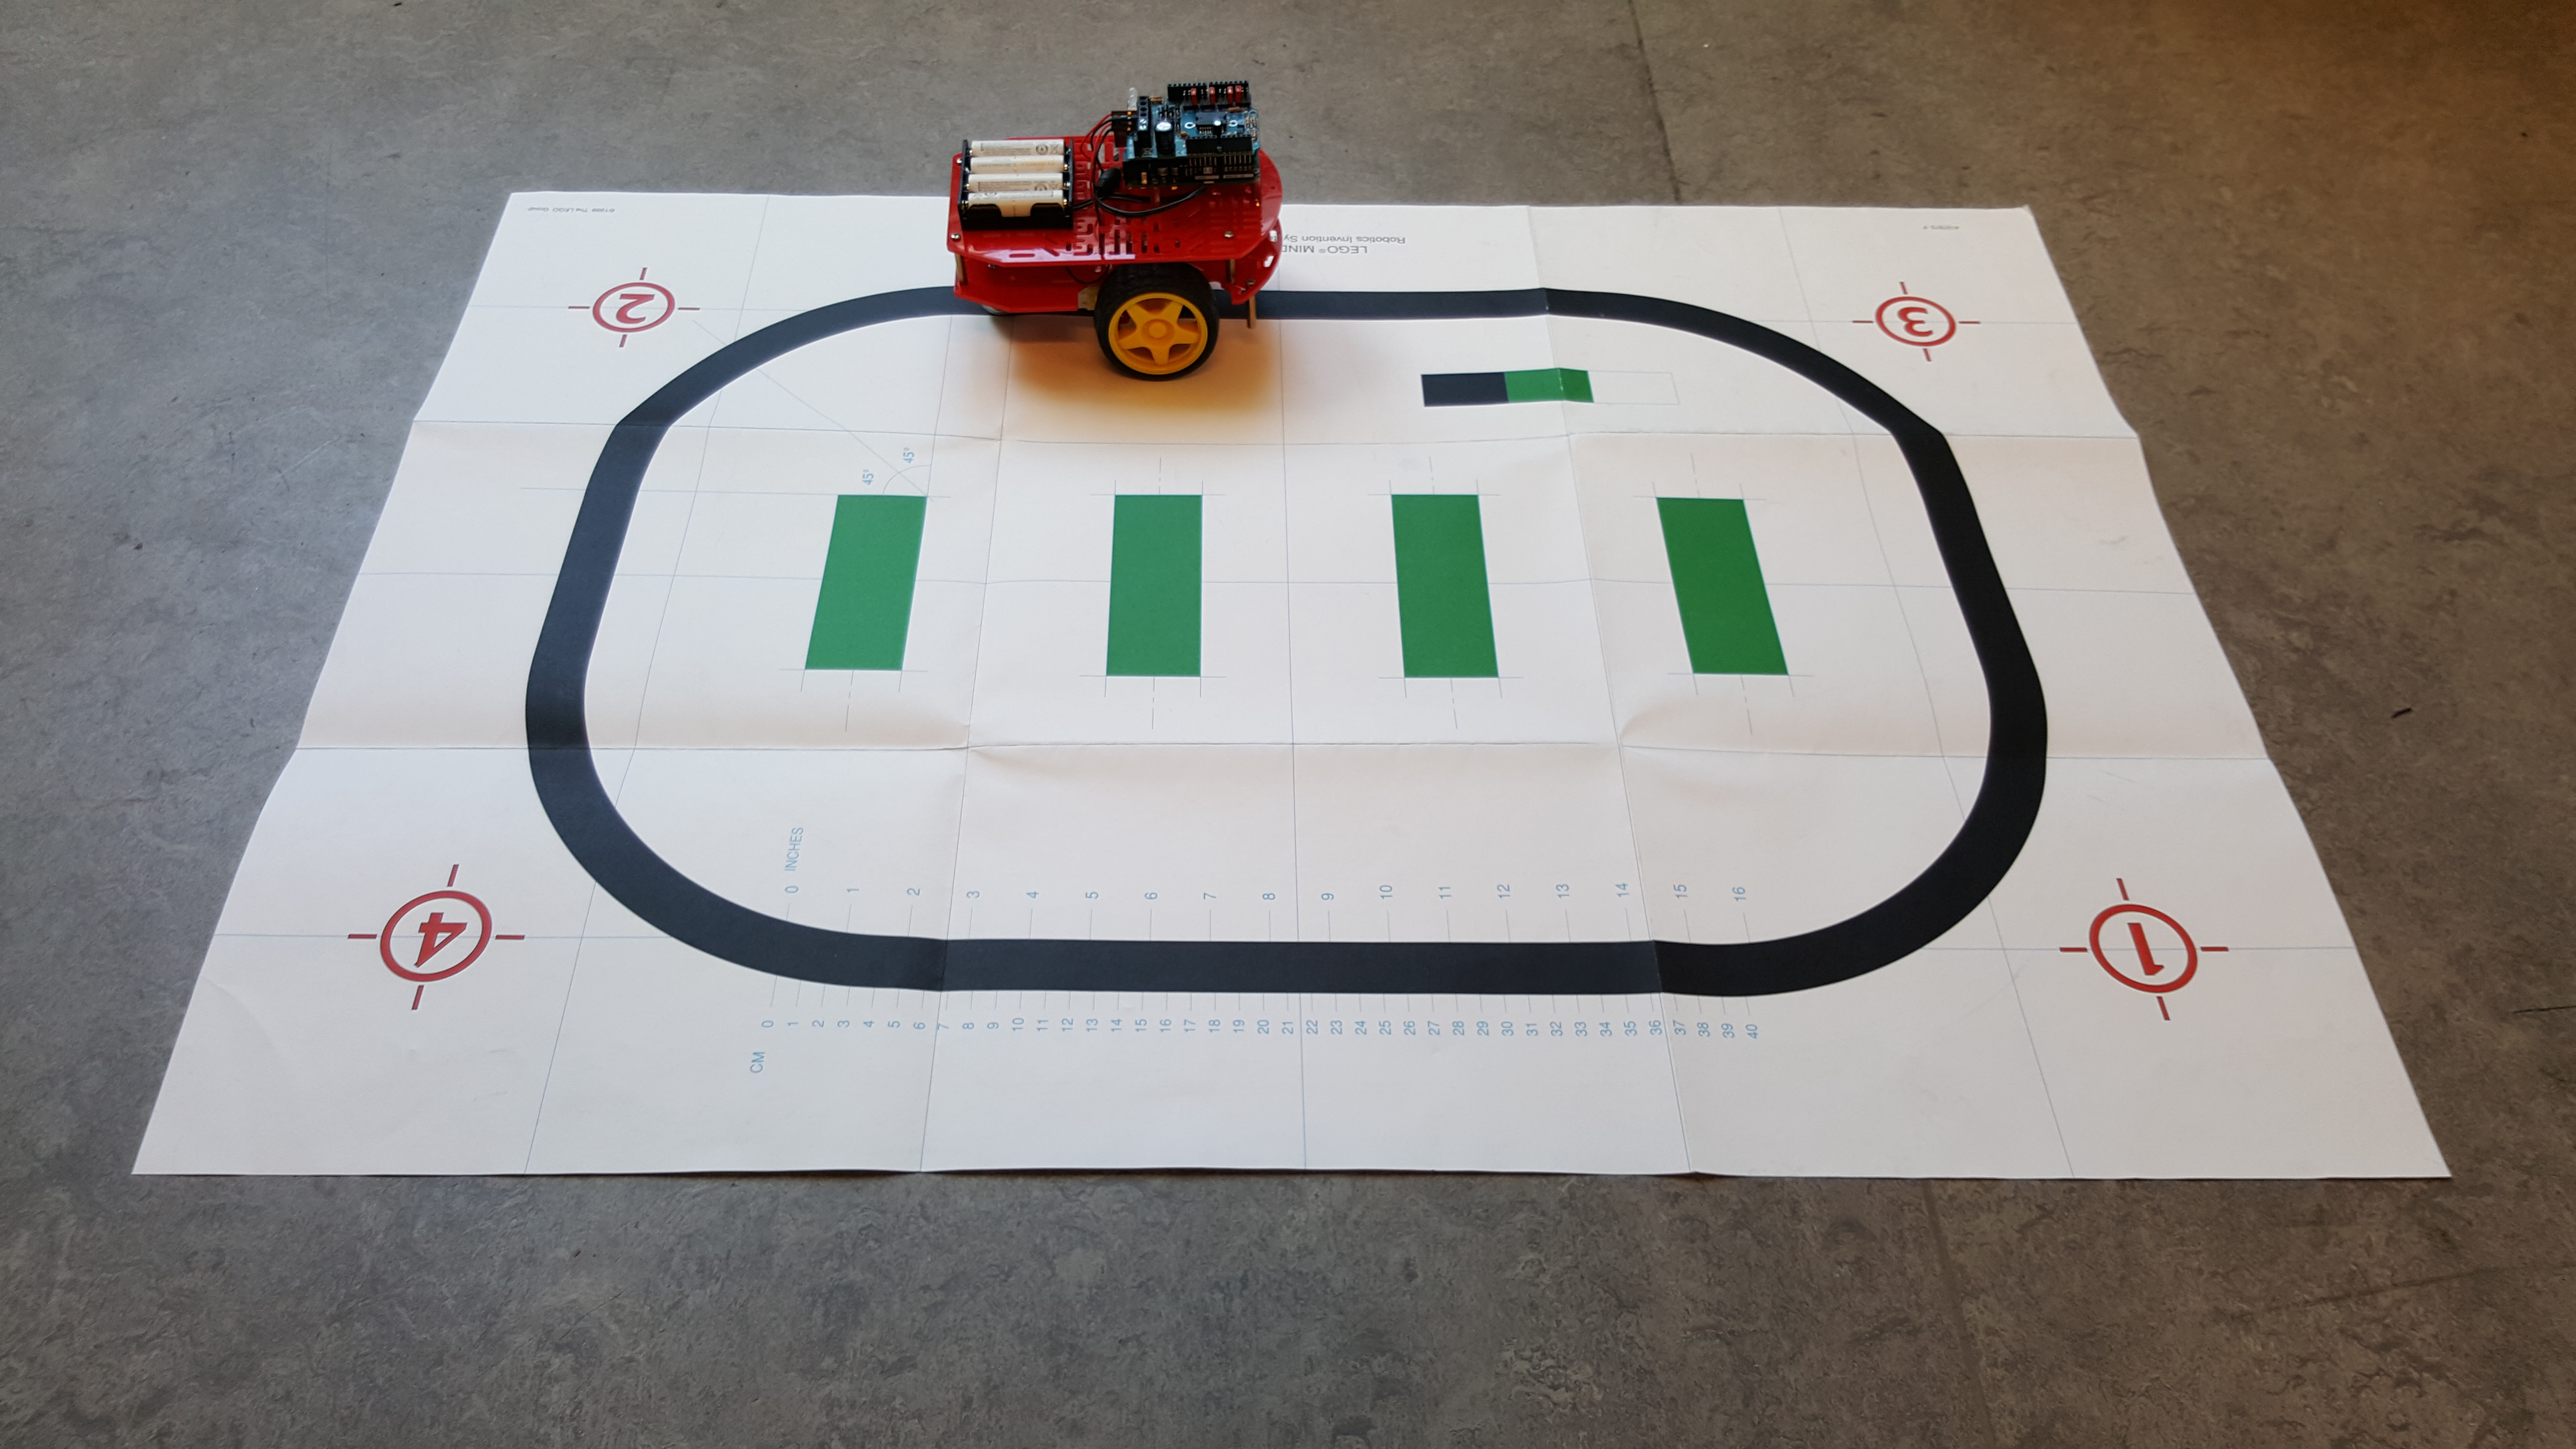
\includegraphics[width=0.6\textwidth]{figures/testMedEnSensor.png}
  \caption{Den inledende software løsning til linetrackinging med 1 sensor.}
  \label{init_software}
\end{figure}


